\documentclass[]{standalone}

\usepackage{tikz}
\usetikzlibrary{automata, positioning, arrows}

\begin{document}
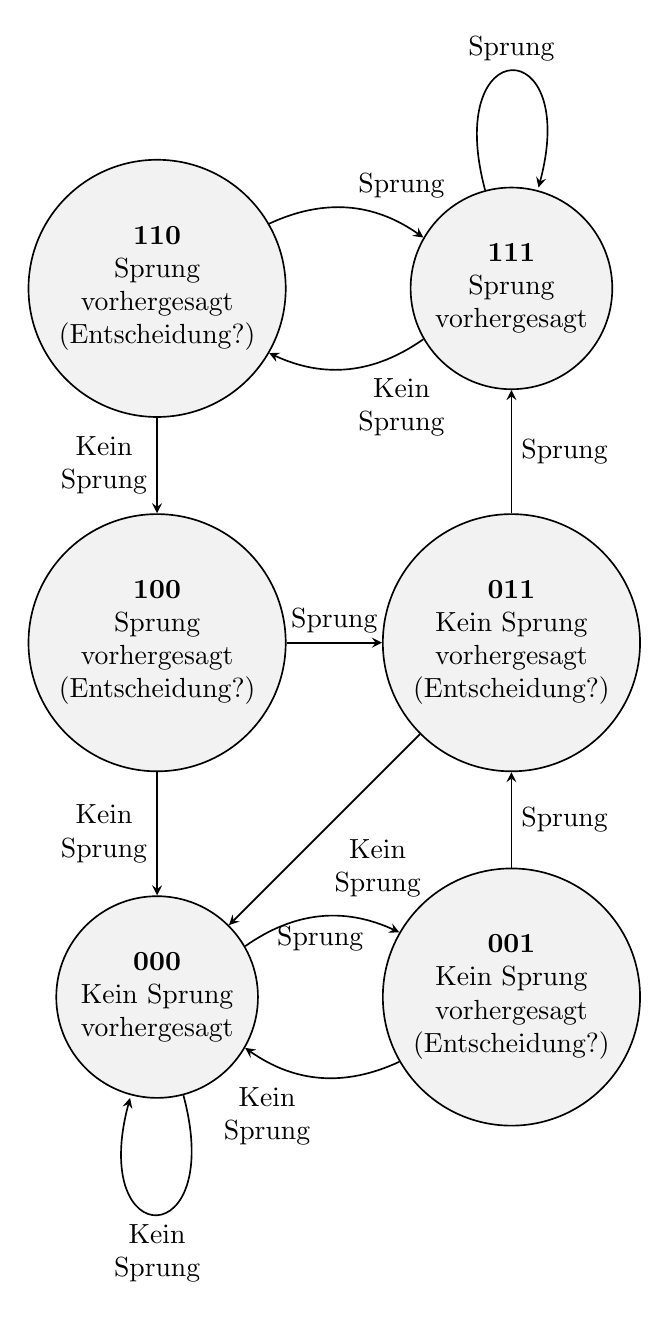
\begin{tikzpicture}[node distance=4.5cm]
	\tikzstyle{every state}=[semithick, fill=gray!10]
	\tikzstyle{every edge}=[draw,->,>=stealth,auto,semithick]

	\node[state,align=center] (000) {\textbf{000}\\Kein Sprung\\vorhergesagt};
	\node[state,align=center, right of=000] (001) {\textbf{001}\\Kein Sprung\\vorhergesagt\\(Entscheidung?)};
	\node[state,align=center, above of=001] (011) {\textbf{011}\\Kein Sprung\\vorhergesagt\\(Entscheidung?)};
	\node[state,align=center, above of=011] (111) {\textbf{111}\\Sprung\\vorhergesagt};
	\node[state,align=center, left of=111] (110) {\textbf{110}\\Sprung\\vorhergesagt\\(Entscheidung?)};
	\node[state,align=center, above of=000] (100) {\textbf{100}\\Sprung\\vorhergesagt\\(Entscheidung?)};

	\draw (000) edge[loop below] node[align=center] {Kein\\Sprung} (000)
	edge[bend left] node[align=center,below] {Sprung} (001);
	\draw (001) edge[bend left] node[align=center] {Kein\\Sprung} (000)
	edge node[align=center,right] {Sprung} (011);
	\draw (011) edge node[align=center] {Kein\\Sprung} (000)
	edge node[align=center,right] {Sprung} (111);
	\draw (111) edge[loop above] node[align=center] {Sprung} (111)
	edge[bend left] node[align=center] {Kein\\Sprung} (110);
	\draw (110) edge[bend left] node[align=center] {Sprung} (111)
	edge node[align=center,left] {Kein\\Sprung} (100);
	\draw (100) edge node[align=center,left] {Kein\\Sprung} (000)
	edge node[align=center] {Sprung} (011);
\end{tikzpicture}
\end{document}
